
\section{Causal broadcast\\for large and dynamic systems}
\label{sec:proposal}

In this section, we introduce \CBROADCAST (stands for Preventive Causal
broadcast), a causal broadcast protocol that breaks the scalability barrier for
large and dynamic systems.  Our approach is preventive: instead of repairing
causal order violations or reordering received messages, it simply makes sure
that messages never arrive out of causal order. Processes can immediately
deliver messages upon receipt. This not only removes most of control information
piggybacked in broadcast messages, but also leads to constant delivery execution
time. Protocols and applications can finally afford causal broadcast in large
and dynamic systems without loss of efficiency.

\subsection{Model}

A distributed system comprises processes. Processes can communicate with each
other using messages. They may not have full knowledge of the membership, for
maintenance is too costly in large and dynamic systems. Instead, processes build
overlay networks with local partial view the size of which is generally much
smaller than the actual size of the
system~\cite{bertier-d2ht,jelasity2007gossip,jelasity2009tman}. Overlay networks
can be built on top of other overlay networks.  For the rest of this paper, we
will use the terms of distributed systems, overlay networks, or networks
indifferently.

\begin{definition}[Overlay network]
  An overlay network $G$ is a pair $\langle P,\, E\rangle$ where $P$ is a set of
  processes, and $E$ is a set of links $E: P\times P$. An overlay network is
  static when $P$ and $E$ are immutable, otherwise it
  is dynamic.
\end{definition}

\begin{definition}[Process]
  A process runs a set of instructions sequentially and communicates
  with other processes using message passing. \\
  A process' neighborhood is the set of links departing from it. \\
  A process~A can send messages to another process~B in its neighborhood:
  $s_{AB}(m)$; receive a message from another process~C that has Process~A as
  neighbor:
  $r_{AC}(m)$. \\
  A process is faulty if it crashes, otherwise it is correct. We do not consider
  byzantine processes.
\end{definition}


\begin{definition}[Unpartitioned network]
  A network is unpartitioned if and only if for any pair of correct processes,
  there exist a path -- a link or a sequence of links -- of correct processes
  between them. We only consider unpartitioned overlay networks.
\end{definition}

Causal broadcast is a communication primitive that relies on reliable broadcast
to send messages to all processes in the system.


\begin{definition}[Uniform reliable broadcast]
  When a process~A broadcasts a message $b_A(m)$, each correct process~B in the
  network eventually receives it $r_B(m)$ and delivers it $d_B(m)$.
  Uniform reliable broadcast guarantees 3 properties: \\
  \textbf{Validity:} If a correct process broadcasts a message, then it
  eventually delivers it. \\
  \textbf{Uniform Agreement:} If a process -- correct or not -- delivers a
  message, then all correct processes eventually deliver it. \\
  \textbf{Uniform Integrity:} A process delivers a message at most once, and
  only if it was previously broadcast.
\end{definition}

\begin{algorithm}
  \SetKwProg{Function}{function}{}{}
\SetKwProg{Upon}{upon}{}{}
\SetKwProg{Initially}{INITIALLY:}{}{}
\SetKwProg{Dissemination}{DISSEMINATION:}{}{}

\small

\DontPrintSemicolon
\LinesNumbered

\Initially {} {
  $Q$ \tcp*{$p$'s neighborhood}
  $received \leftarrow \varnothing$ \tcp*{To detect double receipts}
}

\BlankLine

\Dissemination{}{
  
  \Function{\textsc{R-broadcast}($m$) \tcp*[f]{$b_p(m)$}} { 
    $received \leftarrow received \cup m$ \;
    \lForEach {$q \in Q$} {\textsc{sendTo}($q,\, m$)}
    \textsc{R-deliver}($m$) \tcp*{$d_p(m)$}
  }

  \BlankLine
  
  \Upon{\textsc{receive}($m$)}{
    \If {$m \not \in received$} {
      $received \leftarrow received \cup m$ \;
      \lForEach {$q \in Q$} {\textsc{sendTo}($q,\, m$) \tcp*[f]{forward}}
      \textsc{R-deliver}($m$) \tcp*{$d_p(m)$}
    }
  }
  
}


%%% Local Variables:
%%% mode: latex
%%% TeX-master: "../paper"
%%% End:

  \caption{\label{algo:reliablebroadcast}R-broadcast at Process $p$.}
\end{algorithm}

Algorithm~\ref{algo:reliablebroadcast} shows the instructions of a uniform
reliable broadcast. It uses a structure that keeps track of received messages in
order to deliver them at most once.  Since processes may not have full
membership knowledge, processes must forward broadcast messages. Since the
network does not have partitions, processes either receive the message directly
from the broadcaster or transitively. Thus, all correct processes eventually
deliver all messages exactly once. R-broadcast ensures validity, uniform
agreement, and uniform integrity.

Causal broadcast is a reliable broadcast that also ensures a specific ordering
among message deliveries.  To define a delivery order among messages, we define
time in a logical sense using Lamport's definition~\cite{lamport1978time}.

\begin{definition}[Happen before~\cite{lamport1978time}]
  Happen before is a transitive, irreflexive, and antisymmetric relation
  $\rightarrow$ that defines a strict partial order of events.  The sending of a
  message always precedes its receipt.
\end{definition}

To order messages broadcast by every process, we define causal order.

\begin{definition}[Causal order]
  The delivery order of messages follows the happen before relationships of
  corresponding broadcasts:
  $\forall A,\,B,\,C,\, b_A(m) \rightarrow b_B(m') \implies d_C(m) \rightarrow
  d_C(m')$
\end{definition}

\begin{definition}[Causal broadcast]
  Causal broadcast is a uniform reliable broadcast ensuring causal order.
\end{definition}

\begin{theorem}[\label{theo:flooding}Constraint flooding in deterministic
  overlay networks is causal~\cite{friedman2004causal}]
  In static networks, a broadcast protocol is causal if it uses FIFO links,
  forwards all broadcast messages exactly once, and uses all its outgoing links.
\end{theorem}

From Theorem~\ref{theo:flooding}, reliable broadcast from
Algorithm~\ref{algo:reliablebroadcast} is causal if communication links employed
to communicate with neighbors in $Q$ are FIFO. This holds only for static
networks where $Q$ is immutable. In practice, processes can join, leave, add or
remove links to neighbors from $Q$ at any time.

\begin{lemma}[R-broadcast is causal in dynamic systems subject to
  removals\label{lem:removals}]
  R-broadcast using FIFO links is a causal broadcast in dynamic systems where
  processes can leave the system or links can be removed.
\end{lemma}

\begin{proof}
  Removing a process from the network and removing all the incoming and outgoing
  links of this process is equivalent. Since we assume that removals do not
  create network partitions\footnote{It may create partitions infringing the
    uniform agreement property. Network partitioning constitutes an orthogonal
    problem that we do not address in this paper.}, all correct processes
  eventually receive all broadcast messages. In addition, removing a link or a
  process does not reorder causally related messages. Hence, each process
  receives and delivers each broadcast message in causal order as in static
  systems.
\end{proof}

Link removals and process departures do not endanger broadcast properties.
However, Figure~\ref{fig:preventiveproblem} shows that adding links may lead to
causal order violations. The next section describes \CBROADCAST, a causal
broadcast that handles all dynamicity.

\subsection{Causal order in dynamic systems}

\begin{figure*}
  \begin{center}
    \subfloat[Part A][\label{fig:preventivesolveA}Process~A broadcasts $a$.]
    {
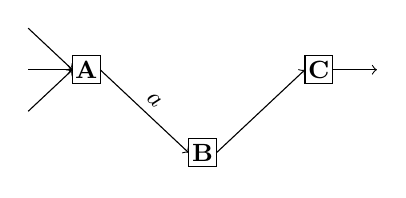
\begin{tikzpicture}[scale=1]
  
  \small
  
  \newcommand\X{210/5pt};
  \newcommand\Y{30pt};
  
  \draw[->] ( -0.5*\X, 0.5*\Y) -- ( -5+0*\X, 0*\Y);
  \draw[->] ( -0.5*\X, 0*\Y) -- ( -5+0*\X, 0*\Y);
  \draw[->] ( -0.5*\X, -0.5*\Y) -- ( -5+0*\X, 0*\Y);  

  \draw[fill=white] (0*\X, 0*\Y) node{\textbf{A}} +(-5pt, -5pt) rectangle +(5pt, 5pt);
  \draw[fill=white] (1*\X, -1*\Y) node{\textbf{B}} +(-5pt, -5pt) rectangle +(5pt, 5pt);
  \draw[fill=white] (2*\X,  0*\Y) node{\textbf{C}} +(-5pt, -5pt) rectangle +(5pt, 5pt);

  \draw[->](5+0*\X, 0*\Y) -- node[sloped, above]{$a$} (-5+1*\X, -1*\Y); %% A->B
  \draw[->](5+1*\X, -1*\Y) -- (-5+2*\X, 0*\Y); %% B->D

  \draw[->](5+2*\X, 0*\Y) -- ( 2.5*\X, 0*\Y);
\end{tikzpicture}}
    \hspace{20pt}
    \subfloat[Part B][\label{fig:preventivesolveB}Process~A wants
    to add a link to Process~C. 
    It sends a ping message $\pi$ to Process~C using one of its FIFO links.]
    {
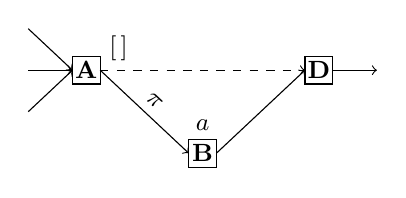
\begin{tikzpicture}[scale=1]
  
  \small
  
  \newcommand\X{210/5pt};
  \newcommand\Y{30pt};
  
  \draw[->] ( -0.5*\X, 0.5*\Y) -- ( -5+0*\X, 0*\Y);
  \draw[->] ( -0.5*\X, 0*\Y) -- ( -5+0*\X, 0*\Y);
  \draw[->] ( -0.5*\X, -0.5*\Y) -- ( -5+0*\X, 0*\Y);  

  \draw[fill=white] (0*\X, 0*\Y) node{\textbf{A}} +(-5pt, -5pt) rectangle +(5pt, 5pt);
  \draw[fill=white] (1*\X, -1*\Y) node{\textbf{B}} +(-5pt, -5pt) rectangle +(5pt, 5pt);
  \draw (1*\X, 5-1*\Y) node[anchor=south]{$a$};
  \draw[fill=white] (2*\X,  0*\Y) node{\textbf{D}} +(-5pt, -5pt) rectangle +(5pt, 5pt);

  \draw[->](5+0*\X, 0*\Y) -- node[sloped, above]{$\pi$} (-5+1*\X, -1*\Y); %% A->B
  \draw[->](5+1*\X, -1*\Y) -- (-5+2*\X, 0*\Y); %% B->D
  
  \draw[->, dashed] (5+0*\X, 0*\Y) node[anchor=south west]{$[\,]$} -- (-5+2*\X, 0*\Y); %% A->B

  \draw[->](5+2*\X, 0*\Y) -- ( 2.5*\X, 0*\Y);
\end{tikzpicture}}
    \hspace{20pt}
    \subfloat[Part C][\label{fig:preventivesolveC}Process~A broadcasts $a'$.
    It does not send it through the new link but buffers it.]
    {
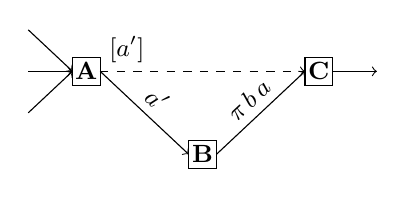
\begin{tikzpicture}[scale=1]
  
  \small
  
  \newcommand\X{210/5pt};
  \newcommand\Y{30pt};
  
  \draw[->] ( -0.5*\X, 0.5*\Y) -- ( -5+0*\X, 0*\Y);
  \draw[->] ( -0.5*\X, 0*\Y) -- ( -5+0*\X, 0*\Y);
  \draw[->] ( -0.5*\X, -0.5*\Y) -- ( -5+0*\X, 0*\Y);  

  \draw[fill=white] (0*\X, 0*\Y) node{\textbf{A}} +(-5pt, -5pt) rectangle +(5pt, 5pt);
  \draw[fill=white] (1*\X, -1*\Y) node{\textbf{B}} +(-5pt, -5pt) rectangle +(5pt, 5pt);
%  \draw (1*\X, 5-1*\Y) node[anchor=south]{$a$};
  \draw[fill=white] (2*\X,  0*\Y) node{\textbf{C}} +(-5pt, -5pt) rectangle +(5pt, 5pt);

  \draw[->](5+0*\X, 0*\Y) -- node[sloped, above]{$a'$} (-5+1*\X, -1*\Y); %% A->B
  \draw[->](5+1*\X, -1*\Y) -- node[sloped, above]{$\pi\,b\,a$} (-5+2*\X, 0*\Y); %% B->D
  
  \draw[->, dashed] (5+0*\X, 0*\Y) node[anchor=south west]{$[a']$} --  (-5+2*\X, 0*\Y); %% A->B

  \draw[->](5+2*\X, 0*\Y) -- ( 2.5*\X, 0*\Y);
\end{tikzpicture}}
    \hspace{20pt}
    \subfloat[Part D][\label{fig:preventivesolveD}Process~C receives
    $\pi$ and replies to $A$.
    The reply $\rho$ can travel by any communication
    mean.]
    {
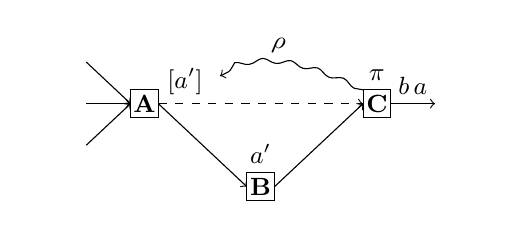
\begin{tikzpicture}[scale=1]
  
  \small
  
  \newcommand\X{210/5pt};
  \newcommand\Y{30pt};

  \draw (-1*\X, 0*\Y);
  \draw (3*\X, 0*\Y);

  
  \draw[->] ( -0.5*\X, 0.5*\Y) -- ( -5+0*\X, 0*\Y);
  \draw[->] ( -0.5*\X, 0*\Y) -- ( -5+0*\X, 0*\Y);
  \draw[->] ( -0.5*\X, -0.5*\Y) -- ( -5+0*\X, 0*\Y);  

  \draw[fill=white] (0*\X, 0*\Y) node{\textbf{A}} +(-5pt, -5pt) rectangle +(5pt, 5pt);
  \draw[fill=white] (1*\X, -1*\Y) node{\textbf{B}} +(-5pt, -5pt) rectangle +(5pt, 5pt);
  \draw (1*\X, 5-1*\Y) node[anchor=south]{$a'$};
  \draw[fill=white] (2*\X,  0*\Y) node{\textbf{C}} +(-5pt, -5pt) rectangle +(5pt, 5pt);
  \draw (2*\X, 5-0*\Y) node[anchor=south]{$\pi$};

  \draw[->](5+0*\X, 0*\Y) -- (-5+1*\X, -1*\Y); %% A->B
  \draw[->](5+1*\X, -1*\Y) -- (-5+2*\X, 0*\Y); %% B->D
  
  \draw[->, dashed] (5+0*\X, 0*\Y) node[anchor=south west]{$[a']$} --  (-5+2*\X, 0*\Y); %% A->B

  \draw[->, decorate, decoration={snake, amplitude=0.3mm}](-5+2*\X, 5+0*\Y)
  to[out=180-25, in=25] node[sloped, above left]{$\rho$}(0.65*\X, 10+0*\Y); 

  \draw[->](5+2*\X, 0*\Y) -- node[anchor=south]{$b\,a$}( 2.5*\X, 0*\Y);
\end{tikzpicture}}
    \hspace{20pt}
    \subfloat[Part E][\label{fig:preventivesolveE}Process~A receives
    Process~C's reply. 
    The former safely empties its buffer to Process~C. 
    Using the new link cannot cause causal order violation anymore.]
    {
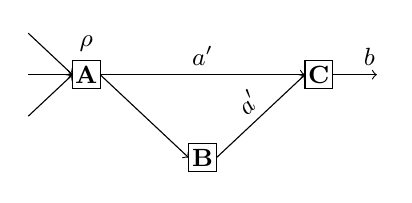
\begin{tikzpicture}[scale=1]
  
  \small
  
  \newcommand\X{210/5pt};
  \newcommand\Y{30pt};
  
  \draw[->] ( -0.5*\X, 0.5*\Y) -- ( -5+0*\X, 0*\Y);
  \draw[->] ( -0.5*\X, 0*\Y) -- ( -5+0*\X, 0*\Y);
  \draw[->] ( -0.5*\X, -0.5*\Y) -- ( -5+0*\X, 0*\Y);  

  \draw[fill=white] (0*\X, 0*\Y) node{\textbf{A}} +(-5pt, -5pt) rectangle +(5pt, 5pt);
  \draw (0*\X, 5-0*\Y) node[anchor=south]{$\rho$};
  \draw[fill=white] (1*\X, -1*\Y) node{\textbf{B}} +(-5pt, -5pt) rectangle +(5pt, 5pt);
  \draw[fill=white] (2*\X,  0*\Y) node{\textbf{C}} +(-5pt, -5pt) rectangle +(5pt, 5pt);

  \draw[->](5+0*\X, 0*\Y) -- (-5+1*\X, -1*\Y); %% A->B
  \draw[->](5+1*\X, -1*\Y) -- node[sloped, above]{$a'$} (-5+2*\X, 0*\Y); %% B->D
  
  \draw[->] (5+0*\X, 0*\Y)  -- node[anchor=south]{$a'$} (-5+2*\X, 0*\Y); %% A->B

  \draw[->](5+2*\X, 0*\Y) -- node[anchor=south west]{$b$}( 2.5*\X, 0*\Y);
\end{tikzpicture}}
    \caption{\label{fig:preventivesolve}\CBROADCAST does not violate causal
      order in dynamic settings.}
  \end{center}
\end{figure*}


\CBROADCAST stands for Preventive Causal broadcast. It prevents causal order
violations by forbidding the usage of new links until proven safe. It
constitutes a powerful yet simple extension
of~\cite{friedman2004causal}. Table~\ref{table:comparison} shows that it
preserves both constant message overhead and constant delivery execution time in
dynamic settings.

Figure~\ref{fig:preventiveproblem} shows that adding links may infringe the
causal order property of causal broadcast.  New links may act as shortcuts for
new messages: new messages that travel through new links may arrive before
preceding messages that took longer paths. To prevent this behavior, we define
the safety of a link. \CBROADCAST uses all and only safe links to disseminate
messages.

\begin{definition}[\label{def:safe}Safe link]
  A link from Process~A to Process~B is safe if and only if Process~B received
  or will receive all messages delivered by Process~A before receiving any
  message that Process~A will deliver:
  $safe_{AB} \equiv \forall m,\, m',\, d_A(m) \rightarrow s_{AB}(m') \implies
  r_B(m) \rightarrow r_{BA}(m')$
\end{definition}

Added links start unsafe. In Figure~\ref{fig:preventiveproblem}, Process~A uses
the link to broadcast $a'$ while it is unsafe: Process~B did not receive $a$
yet, and there was no guarantee that Process~B would receive $a$ before receiving
$a'$ from the new link. In this example, the worst happens and Process~B
receives then delivers $a'$ before $a$ which violates causal order.

The challenge is to make unsafe links safe using local knowledge only. A
straightforward mean for Process~A to achieve this consists in sending all its
delivered messages to Process~B using this unsafe link. This guarantees that any
message delivered by A will be received by B before A starts using the new --
now safe -- link for causal broadcast. However, this is costly both in local
space and generated traffic. Performing an anti-entropy round to extract missing
messages would also be overcostly in terms of generated traffic for it would
require sending the vector of received messages~\cite{demers1987epidemic}.
Instead, Process~A avoid sending most of messages by initiating a ping phase
to Process~B. 

\begin{definition}[Ping phase]
  Ping phase starts when Process~A pings Process~B. Ping messages $\pi$ travel
  using safe links. When Process~B receives this ping, it replies to
  Process~A. Replies $\rho$ travel using any communication mean. Ping phase ends
  when Process~A receives the reply of Process~B.
\end{definition}

\begin{lemma}[\label{lemma:ping}Ping phases acknowledge broadcast receipts]
  A ping phase from Process~A to Process~B acknowledges the receipt by B of all
  messages delivered by Process~A before this ping phase:
  $\forall m,\, d_A(m) \rightarrow s_A(\pi_{AB}) \wedge r_A(\rho_{AB}) \implies
  r_B(m)$
\end{lemma}

\begin{proof}
  Suppose a process~A initiates a ping phase to a process B. Suppose a series of
  messages delivered by Process~A. Process~A sent every of these messages
  exactly once using all its outgoing safe links. Processes that will receive
  these messages either already forwarded them or will forward them in their
  receipt order. Since Process~A's ping travels using safe links after these
  messages, when Process~B receives the ping, it already received all messages
  delivered by Process~A. Process~A receives Process~B's reply after Process~B
  received the ping. Consequently, when Process~A receives Process~B's reply,
  Process~B received all messages delivered by Process~A before the start of
  this ping phase.
\end{proof}

Upon receipt of Process~B's reply, Process~A has the guarantee that Process~B
received all its delivered messages preceding the ping phase. This is not
sufficient, for ping phases take time. Messages delivered during ping phase by
Process~A may not be received by Process~B yet. To fill this gap, Process~A
sends to Process~B the messages it buffered during the ping phase.

\begin{definition}[Buffering]
  Process~A records in a buffer $\mathcal{B}$ all its delivered messages during
  a ping phase to Process~B.
  $\forall m,\, s_A(\pi_{AB}) \rightarrow d_A(m) \wedge d_A(m)\rightarrow
  r_A(\rho_{AB}) \Leftrightarrow m \in \mathcal{B} $
\end{definition}


\begin{lemma}[Ping phase and buffering makes safe links]
  Process~A makes an unsafe link to Process~B safe by completing a ping phase to
  Process~B then finalizing it by sending all delivered messages buffered during
  ping phase using the new link.
\end{lemma}

\begin{proof}
  Suppose a series of messages $m_1 \ldots m_i \ldots m_j$ delivered by a
  process A. Suppose Process~A initiated a ping phase to a process~B after
  delivering $m_i$. Suppose Process~A receives Process~B's reply after $m_j$.
  We must show that when Process~A delivers a message after $m_k$, Process~B
  received or will receive $m_1 \ldots m_j$ before. \\
  From Lemma~\ref{lemma:ping}, when Process~A receives Process~B's reply,
  Process~B received $m_1 \ldots m_i$. \\
  Since Process~A buffered all messages delivered since the beginning of the
  ping phase, the buffer contains $m_{i+1} \ldots m_j$ when the ping phase ends.
  Since links are FIFO, sending messages of this buffer using the new link
  guarantees that Process~B will receive them before receiving any $m_k$
  delivered after $m_j$. The link from Process~A to Process~B became safe.
\end{proof}


\begin{lemma}[\CBROADCAST is causal in dynamic systems subject to
  additions\label{lem:additions}]
  In dynamic systems where processes can join or add links, broadcasting using
  all and only safe FIFO links ensures causal order. Without partition, the
  broadcast is causal.
\end{lemma}

\begin{proof}
  \CBROADCAST ensures \textbf{validity}, \textbf{uniform agreement}, and
  \textbf{uniform integrity},
  for it extends R-broadcast that ensures all 3 properties. \\
  We must show that \CBROADCAST ensures \textbf{causal order}:
  $\forall A,\,B,\,C,\, b_A(m) \rightarrow b_B(m')
  \implies d_C(m) \rightarrow d_C(m')$. \\
  $\forall A,\,B,\, b_A(m) \rightarrow b_B(m') \Leftrightarrow d_B(m)
  \rightarrow d_B(m') \Leftrightarrow d_B(m) \rightarrow s_B(m') \Leftrightarrow
  d_B(m) \rightarrow (\forall C\in Q, s_{BC}(m'))$.
  Since all links in $Q$ are safe links, $r_c(m) \rightarrow r_{CB}(m')$ (see
  Definition~\ref{def:safe}).  Since delivery order follows first receipt order,
  $d_C(m) \rightarrow d_C(m')$. This order on message delivery transitively
  reach all correct processes as long as the network remains unpartitioned.
\end{proof}



\begin{figure*}
  \begin{center}
    \subfloat[part A][\label{fig:bufferproblemA}Slow ping message $\pi$.]
    {
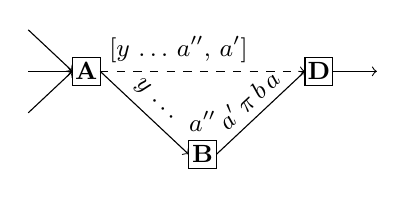
\begin{tikzpicture}[scale=1]
  
  \small
  
  \newcommand\X{210/5pt};
  \newcommand\Y{30pt};
  
  \draw[->] ( -0.5*\X, 0.5*\Y) -- ( -5+0*\X, 0*\Y);
  \draw[->] ( -0.5*\X, 0*\Y) -- ( -5+0*\X, 0*\Y);
  \draw[->] ( -0.5*\X, -0.5*\Y) -- ( -5+0*\X, 0*\Y);  

  \draw[fill=white] (0*\X, 0*\Y) node{\textbf{A}} +(-5pt, -5pt) rectangle +(5pt, 5pt);
  \draw[fill=white] (1*\X, -1*\Y) node{\textbf{B}} +(-5pt, -5pt) rectangle +(5pt, 5pt);
  \draw (1*\X, 5-1*\Y) node[anchor=south]{$a''$};
  \draw[fill=white] (2*\X,  0*\Y) node{\textbf{D}} +(-5pt, -5pt) rectangle +(5pt, 5pt);

  \draw[->, dashed] (5+0*\X, 0*\Y) -- (-5+2*\X, 0*\Y);

  \draw[->](5+0*\X, 0*\Y) node[anchor=south west]{$[y\, \ldots \,a'',\,a']$} -- node[sloped, above]{$y\, \dots$} (-5+1*\X, -1*\Y); %% A->B
  \draw[->](5+1*\X, -1*\Y) -- node[sloped, above]{$a'\,\pi\,b\,a$} (-5+2*\X, 0*\Y); %% B->D

  \draw[->](5+2*\X, 0*\Y) -- ( 2.5*\X, 0*\Y);
\end{tikzpicture}}
    \hspace{20pt}
    \subfloat[part B][\label{fig:bufferproblemB}Process~C crashes.]
    {
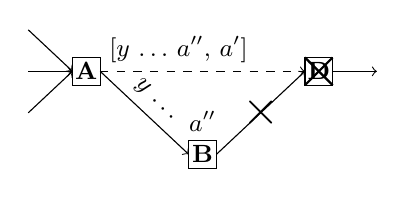
\begin{tikzpicture}[scale=1]
  
  \small
  
  \newcommand\X{210/5pt};
  \newcommand\Y{30pt};
  
  \draw[->] ( -0.5*\X, 0.5*\Y) -- ( -5+0*\X, 0*\Y);
  \draw[->] ( -0.5*\X, 0*\Y) -- ( -5+0*\X, 0*\Y);
  \draw[->] ( -0.5*\X, -0.5*\Y) -- ( -5+0*\X, 0*\Y);  

  \draw[fill=white] (0*\X, 0*\Y) node{\textbf{A}} +(-5pt, -5pt) rectangle +(5pt, 5pt);
  \draw[fill=white] (1*\X, -1*\Y) node{\textbf{B}} +(-5pt, -5pt) rectangle +(5pt, 5pt);
  \draw (1*\X, 5-1*\Y) node[anchor=south]{$a''$};
  \draw[fill=white] (2*\X,  0*\Y) node{\textbf{D}} +(-5pt, -5pt) rectangle +(5pt, 5pt);

  \draw[->, dashed] (5+0*\X, 0*\Y) -- (-5+2*\X, 0*\Y);

  \draw[->](5+0*\X, 0*\Y) node[anchor=south west]{$[y\, \ldots \,a'',\,a']$} -- node[sloped, above]{$y\,\ldots$} (-5+1*\X, -1*\Y); %% A->B
  \draw[->](5+1*\X, -1*\Y) -- % node[sloped, above]{$a'\,\ell\,b\,a$}
  node{\LARGE$\times$}(-5+2*\X, 0*\Y); %% B->D

  \draw[thick] (-5+2*\X, -5+0*\Y) -- (5+2*\X, 5+0*\Y);
  \draw[thick] (-5+2*\X, 5+0*\Y) -- (5+2*\X, -5+0*\Y);

  \draw[->](5+2*\X, 0*\Y) -- ( 2.5*\X, 0*\Y);
\end{tikzpicture}}
    \hspace{20pt}
    \subfloat[part C][\label{fig:bufferproblemC}Reply $\rho$ fails.]
    {
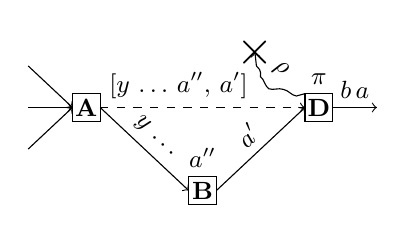
\begin{tikzpicture}[scale=1]
  
  \small
  
  \newcommand\X{210/5pt};
  \newcommand\Y{30pt};
  
  \draw[->] ( -0.5*\X, 0.5*\Y) -- ( -5+0*\X, 0*\Y);
  \draw[->] ( -0.5*\X, 0*\Y) -- ( -5+0*\X, 0*\Y);
  \draw[->] ( -0.5*\X, -0.5*\Y) -- ( -5+0*\X, 0*\Y);  

  \draw[fill=white] (0*\X, 0*\Y) node{\textbf{A}} +(-5pt, -5pt) rectangle +(5pt, 5pt);
  \draw[fill=white] (1*\X, -1*\Y) node{\textbf{B}} +(-5pt, -5pt) rectangle +(5pt, 5pt);
  \draw (1*\X, 5-1*\Y) node[anchor=south]{$a''$};
  \draw[fill=white] (2*\X,  0*\Y) node{\textbf{D}} +(-5pt, -5pt) rectangle +(5pt, 5pt);
  \draw (2*\X, 5-0*\Y) node[anchor=south]{$\pi$};

  \draw[->, dashed] (5+0*\X, 0*\Y) -- (-5+2*\X, 0*\Y);

  \draw[->](5+0*\X, 0*\Y) node[anchor=south west]{$[y\, \ldots \,a'',\,a']$} -- node[sloped, above]{$y\,\ldots$} (-5+1*\X, -1*\Y); %% A->B
  \draw[->](5+1*\X, -1*\Y) -- node[sloped, above]{$a'$} (-5+2*\X, 0*\Y); %% B->D

  \draw[->, decorate, decoration={snake, amplitude=0.3mm}](-5+2*\X, 5+0*\Y)
  to[out=180, in=-90] node[sloped, above]{$\rho$}(1.45*\X, 20+0*\Y)
  node{\LARGE$\times$}; 


  \draw[->](5+2*\X, 0*\Y) -- node[above]{$b\,a$}( 2.5*\X, 0*\Y);
\end{tikzpicture}}
    \caption{\label{fig:bufferproblem}Buffers may grow unbounded due to network
      conditions.}
  \end{center}
\end{figure*}



\begin{algorithm}
  
\SetKwProg{Function}{function}{}{}
\SetKwProg{Upon}{upon}{}{}
\SetKwProg{Initially}{INITIALLY:}{}{}
\SetKwProg{Dissemination}{DISSEMINATION:}{}{}
\SetKwProg{Safety}{SAFETY:}{}{}

\small

\DontPrintSemicolon
\LinesNumbered

\Initially {} {
  $Q$ \tcp*{$p$'s neighborhood, FIFO channels}
  $B \leftarrow \varnothing$ \tcp*{Buffers of messages}
}

\BlankLine

\Safety {} {
  \Upon{\textsc{open}($q$)} {
    \If{$|Q|>1$} {
      $Q \leftarrow Q \setminus q$ \;
      $B[q] \leftarrow \varnothing$ \;
      $\textsc{sendLocked}(p,\, q)$ \;
    }
  }
  
  \BlankLine
  
  \Upon{\textsc{receiveLocked}($from, \, to$) \tcp*[f]{$to=p$}} {
    $\textsc{sendAck}(from,\, to)$ \;
  }
  
  \BlankLine

  \Upon{\textsc{receiveAck}($from,\, to$) \tcp*[f]{$from=p$}} {
    \If {$to \in B$} {
      \lForEach {$m \in B[to]$} {$\textsc{sendTo}(to,\, m)$}
      $B \leftarrow B \setminus to$ \;
      $Q \leftarrow Q \cup to$ \;
    }
  }

  \BlankLine

  \Upon{\textsc{close}($q$)} {
    $B \leftarrow B \setminus q$ \;
  }

}

\BlankLine

\Dissemination {} {

  \Function{\textsc{FBC-broadcast}$^+$($m$) \tcp*[f]{$b_p(m)$}} {    
    \lForEach {$q \in B$} {$B[q] \leftarrow B[q] \cup m$ \tcp*[f]{Buffers}}
    $\textsc{R-broadcast}(m)$ \;
  }
  
  \BlankLine
  
  \Upon{\textsc{R-deliver}($m$)} {
    \lForEach {$q \in B$} {$B[q] \leftarrow B[q] \cup m$ \tcp*[f]{Buffers}}
    $\textsc{FBC-deliver}^+(m)$ \tcp*{$d_p(m)$}
  }

}


%%% Local Variables:
%%% mode: latex
%%% TeX-master: "../paper"
%%% End:

  \caption{\label{algo:bufferbroadcast}\CBROADCAST at Process $p$.}
\end{algorithm}


Algorithm~\ref{algo:bufferbroadcast} shows a small set of instructions that
implement safe links.  Figure~\ref{fig:preventivesolve} shows on an example how
it solves causal order violations. In Figure~\ref{fig:preventivesolveA},
Process~A broadcasts $a$.  In Figure~\ref{fig:preventivesolveB}, Process~A wants
to add a link to Process~C. It sends a ping message $\pi$ to Process~C (see
Line~\ref{line:sendlocked}) and awaits for the latter's reply.  We leave aside
the implementation of this send function (e.g. broadcast or routing).  While
awaiting, Process~A keeps its normal functioning and maintain a buffer of
messages associated with the unsafe link (see Line~\ref{line:bufferforward}). In
Figure~\ref{fig:preventivesolveC}, Process~A broadcasts another message $a'$. It
sends it normally to Process~B but does not send it to Process~C
directly. Instead, it buffers it. In Figure~\ref{fig:preventivesolveD},
Process~C receives Process~A's ping message $\pi$. Since links are FIFO, it
implicitly means that Process~C also received $a$. Process~C sends a reply
$\rho$ to Process~A (see Line~\ref{line:sendack}). $\rho$ can travel through any
communication mean. In Figure~\ref{fig:preventivesolveE}, Process~A receives
$\rho$. Consequently, Process~A knows that Process~C received and delivered at
least $a$ and all preceding messages. It empties the buffer of messages to
Process~C (see Line~\ref{line:emptybuffer}). Afterwards, the new link is
safe. Process~A uses the new link normally.



\begin{figure*}
  \begin{center}
    \subfloat[Part A][\label{fig:buffersolveA}
    Process~A wanted to add a link to Process~C after having
    broadcast $a$. Afterwards, it broadcast $a'$ and $a''$.]
    {
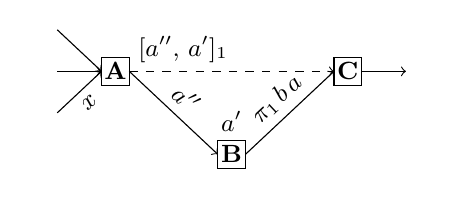
\begin{tikzpicture}[scale=1]
  
  \small
  
  \newcommand\X{210/5pt};
  \newcommand\Y{30pt};

  \draw (-0.75*\X, 0*\Y);
  \draw (2.75*\X, 0*\Y);

  
  \draw[->] ( -0.5*\X, 0.5*\Y) -- ( -5+0*\X, 0*\Y);
  \draw[->] ( -0.5*\X, 0*\Y) -- ( -5+0*\X, 0*\Y);
  \draw[->] ( -0.5*\X, -0.5*\Y) -- node[below,sloped]{$x$} ( -5+0*\X, 0*\Y);  

  \draw[fill=white] (0*\X, 0*\Y) node{\textbf{A}} +(-5pt, -5pt) rectangle +(5pt, 5pt);
  \draw[fill=white] (1*\X, -1*\Y) node{\textbf{B}} +(-5pt, -5pt) rectangle +(5pt, 5pt);
  \draw (1*\X, 5-1*\Y) node[anchor=south]{$a'$};
  \draw[fill=white] (2*\X,  0*\Y) node{\textbf{C}} +(-5pt, -5pt) rectangle +(5pt, 5pt);

  \draw[->, dashed] (5+0*\X, 0*\Y) -- (-5+2*\X, 0*\Y);

  \draw[->](5+0*\X, 0*\Y) node[anchor=south west]{$[a'',\,a']_1$} -- 
  node[sloped, above]{$a''$} (-5+1*\X, -1*\Y); %% A->B
  \draw[->](5+1*\X, -1*\Y) -- node[sloped, above]{$\pi_1\,b\,a$} (-5+2*\X, 0*\Y); %% B->D

  \draw[->](5+2*\X, 0*\Y) -- ( 2.5*\X, 0*\Y);
\end{tikzpicture}}
    \hspace{20pt}
    \subfloat[Part B][\label{fig:buffersolveB}
    Process~A receives, delivers, and forwards $x$. Since the buffer size would 
    exceed the maximal boundary, it resets the buffer with a new counter and
    sends a ping message with this counter. In the meantime, Process~C
    receives $\pi_1$ and sends the corresponding reply $\rho_1$.]
    {
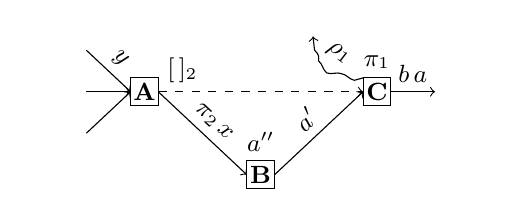
\begin{tikzpicture}[scale=1]
  
  \small
  
  \newcommand\X{210/5pt};
  \newcommand\Y{30pt};

  \draw (-1*\X, 0*\Y);
  \draw (3*\X, 0*\Y);

  
  \draw[->] ( -0.5*\X, 0.5*\Y) -- node[sloped, above]{$y$}( -5+0*\X, 0*\Y);
  \draw[->] ( -0.5*\X, 0*\Y) -- ( -5+0*\X, 0*\Y);
  \draw[->] ( -0.5*\X, -0.5*\Y) -- ( -5+0*\X, 0*\Y);  

  \draw[fill=white] (0*\X, 0*\Y) node{\textbf{A}} +(-5pt, -5pt) rectangle +(5pt, 5pt);
  \draw[fill=white] (1*\X, -1*\Y) node{\textbf{B}} +(-5pt, -5pt) rectangle +(5pt, 5pt);
  \draw (1*\X, 5-1*\Y) node[anchor=south]{$a''$};
  \draw[fill=white] (2*\X,  0*\Y) node{\textbf{C}} +(-5pt, -5pt) rectangle +(5pt, 5pt);
  \draw (2*\X, 5-0*\Y) node[anchor=south]{$\pi_1$};

  \draw[->, dashed] (5+0*\X, 0*\Y) -- (-5+2*\X, 0*\Y);

  \draw[->](5+0*\X, 0*\Y) node[anchor=south west]{$[\,]_2$} -- 
  node[sloped, above]{$\pi_2\,x$} (-5+1*\X, -1*\Y); %% A->B
  \draw[->](5+1*\X, -1*\Y) -- node[sloped, above]{$a'$} (-5+2*\X, 0*\Y); %% B->D

  \draw[->, decorate, decoration={snake, amplitude=0.3mm}](-5+2*\X, 5+0*\Y)
  to[out=180, in=-90] node[sloped, above]{$\rho_1$}(1.45*\X, 20+0*\Y);
%  node{\LARGE$\times$}; 

  \draw[->](5+2*\X, 0*\Y) -- node[above]{$b\,a$}( 2.5*\X, 0*\Y);
\end{tikzpicture}}
    \hspace{20pt}
    \subfloat[Part C][\label{fig:buffersolveC}
    Process~A forwards $y$ and buffers it. It also
    receives $\rho_1$ but no buffers exist with this counter. Process~A 
    simply discards $\rho_1$.]
    {
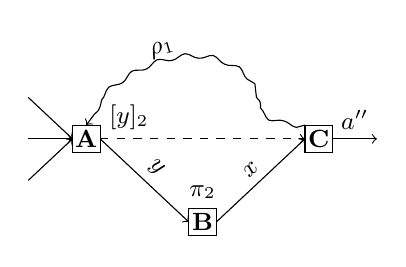
\begin{tikzpicture}[scale=1]
  
  \small
  
  \newcommand\X{210/5pt};
  \newcommand\Y{30pt};
  
  \draw[->] ( -0.5*\X, 0.5*\Y) -- ( -5+0*\X, 0*\Y);
  \draw[->] ( -0.5*\X, 0*\Y) -- ( -5+0*\X, 0*\Y);
  \draw[->] ( -0.5*\X, -0.5*\Y) -- ( -5+0*\X, 0*\Y);  

  \draw[fill=white] (0*\X, 0*\Y) node{\textbf{A}} +(-5pt, -5pt) rectangle +(5pt, 5pt);
  \draw[fill=white] (1*\X, -1*\Y) node{\textbf{B}} +(-5pt, -5pt) rectangle +(5pt, 5pt);
  \draw (1*\X, 5-1*\Y) node[anchor=south]{$\pi_2$};
  \draw[fill=white] (2*\X,  0*\Y) node{\textbf{C}} +(-5pt, -5pt) rectangle +(5pt, 5pt);
%  \draw (2*\X, 5-0*\Y) node[anchor=south]{$\ell_1$};

  \draw[->, dashed] (5+0*\X, 0*\Y) -- (-5+2*\X, 0*\Y);

  \draw[->](5+0*\X, 0*\Y) node[anchor=south west]{$[y]_2$} -- 
  node[sloped, above]{$y$}
  (-5+1*\X, -1*\Y); %% A->B
  \draw[->](5+1*\X, -1*\Y) -- node[sloped, above]{$x$} (-5+2*\X, 0*\Y); %% B->D

  \draw[decorate, decoration={snake, amplitude=0.3mm}](-5+2*\X, 5+0*\Y)
  to[out=180, in=-90] (1.45*\X, 20+0*\Y);
  \draw[->, decorate, decoration={snake, amplitude=0.3mm}](1.45*\X, 20+0*\Y)
  to[out=90+45, in=90-35] node[sloped, above]{$\rho_1$}(0*\X, 5+0*\Y);
%  node{\LARGE$\times$}; 

  \draw[->](5+2*\X, 0*\Y) -- node[above]{$a''$}( 2.5*\X, 0*\Y);
\end{tikzpicture}}
    \hspace{20pt}
    \subfloat[Part D][\label{fig:buffersolveD}
    Process~C receives $\pi_2$ and sends the corresponding
    reply $\rho_2$.]
    {
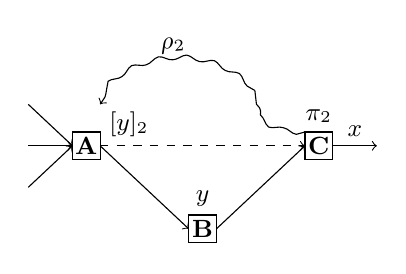
\begin{tikzpicture}[scale=1]
  
  \small
  
  \newcommand\X{210/5pt};
  \newcommand\Y{30pt};
  
  \draw[->] ( -0.5*\X, 0.5*\Y) -- ( -5+0*\X, 0*\Y);
  \draw[->] ( -0.5*\X, 0*\Y) -- ( -5+0*\X, 0*\Y);
  \draw[->] ( -0.5*\X, -0.5*\Y) -- ( -5+0*\X, 0*\Y);  

  \draw[fill=white] (0*\X, 0*\Y) node{\textbf{A}} +(-5pt, -5pt) rectangle +(5pt, 5pt);
  \draw[fill=white] (1*\X, -1*\Y) node{\textbf{B}} +(-5pt, -5pt) rectangle +(5pt, 5pt);
  \draw (1*\X, 5-1*\Y) node[anchor=south]{$y$};
  \draw[fill=white] (2*\X,  0*\Y) node{\textbf{C}} +(-5pt, -5pt) rectangle +(5pt, 5pt);
  \draw (2*\X, 5-0*\Y) node[anchor=south]{$\pi_2$};

  \draw[->, dashed] (5+0*\X, 0*\Y) -- (-5+2*\X, 0*\Y);

  \draw[->](5+0*\X, 0*\Y) node[anchor=south west]{$[y]_2$} -- 
%  node[sloped, above]{$y$}
  (-5+1*\X, -1*\Y); %% A->B
  \draw[->](5+1*\X, -1*\Y) --
  %node[sloped, above]{$a'''$}
  (-5+2*\X, 0*\Y); %% B->D

  \draw[decorate, decoration={snake, amplitude=0.3mm}](-5+2*\X, 5+0*\Y)
  to[out=180, in=-90] (1.45*\X, 20+0*\Y);
  \draw[->, decorate, decoration={snake, amplitude=0.3mm}](1.45*\X, 20+0*\Y)
  to[out=90+45, in=90-35] node[sloped, above]{$\rho_2$}(5+0*\X, 15+0*\Y);
%  node{\LARGE$\times$}; 

  \draw[->](5+2*\X, 0*\Y) -- node[above]{$x$}( 2.5*\X, 0*\Y);
\end{tikzpicture}}
    \hspace{20pt}
    \subfloat[Part E][\label{fig:buffersolveE}
    Process~A receives $\rho_2$. It empties the
    buffer with the corresponding counter. Now,  the direct link
    to Process~C is safe. Process~A uses it normally.]
    {
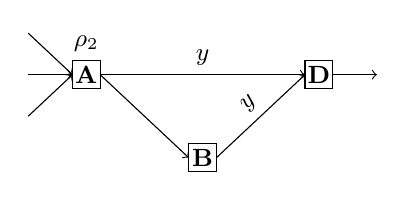
\begin{tikzpicture}[scale=1]
  
  \small
  
  \newcommand\X{210/5pt};
  \newcommand\Y{30pt};
  
  \draw[->] ( -0.5*\X, 0.5*\Y) -- ( -5+0*\X, 0*\Y);
  \draw[->] ( -0.5*\X, 0*\Y) -- ( -5+0*\X, 0*\Y);
  \draw[->] ( -0.5*\X, -0.5*\Y) -- ( -5+0*\X, 0*\Y);  

  \draw[fill=white] (0*\X, 0*\Y) node{\textbf{A}} +(-5pt, -5pt) rectangle +(5pt, 5pt);
  \draw (0*\X, 5-0*\Y) node[anchor=south]{$\rho_2$};
  \draw[fill=white] (1*\X, -1*\Y) node{\textbf{B}} +(-5pt, -5pt) rectangle +(5pt, 5pt);

  \draw[fill=white] (2*\X,  0*\Y) node{\textbf{D}} +(-5pt, -5pt) rectangle +(5pt, 5pt);
%  \draw (2*\X, 5-0*\Y) node[anchor=south]{$\ell_2$};

  \draw[->] (5+0*\X, 0*\Y) -- node[above]{$y$} (-5+2*\X, 0*\Y);

  \draw[->](5+0*\X, 0*\Y) -- (-5+1*\X, -1*\Y); %% A->B
  \draw[->](5+1*\X, -1*\Y) -- node[sloped, above]{$y$} (-5+2*\X, 0*\Y); %% B->D

  % \draw[decorate, decoration={snake, amplitude=0.3mm}](-5+2*\X, 5+0*\Y)
  % to[out=180, in=-90] (1.45*\X, 20+0*\Y);
  % \draw[->, decorate, decoration={snake, amplitude=0.3mm}](1.45*\X, 20+0*\Y)
  % to[out=90+45, in=90-35] node[sloped, above]{$\alpha_2$}(0*\X, 5+0*\Y);
%  node{\LARGE$\times$}; 

  \draw[->](5+2*\X, 0*\Y) -- ( 2.5*\X, 0*\Y);
\end{tikzpicture}}
    \caption{\label{fig:buffersolve}Buffers become bounded. We allow only 2
      elements in each buffer.}
  \end{center}
\end{figure*}


\begin{theorem}[\CBROADCAST is a causal broadcast]
  \CBROADCAST is a causal broadcast in both static and dynamic network settings.
\end{theorem}

\begin{proof}
  For static networks, it comes from~\cite{friedman2004causal}. For dynamic
  networks, it comes from Lemmas~\ref{lem:removals}~and~\ref{lem:additions}.
\end{proof}

\subsection{Bounding space consumption}

Algorithm~\ref{algo:bufferbroadcast} ensures causal delivery of messages even in
dynamic network settings. Compared to the original causal broadcast for static
networks~\cite{friedman2004causal}, it uses an additional local structure:
buffers of messages. It associates a buffer to each new unsafe link. We assumed
that the size of these buffer stays small in general, for it depends on the time
taken by the ping phase which is assumed short. However, network conditions may
invalidate this assumption. Figure~\ref{fig:bufferproblem} depicts scenarios
where buffers grow out of acceptable boundaries. In
Figure~\ref{fig:bufferproblemA}, the issue comes from high transmission delays
from Process~A to Process~B, and from Process~B to Process~C compared to the
number of messages to broadcast and forward. The ping message $\pi$ did not
reach Process~C yet that the buffer contains a lot of messages. In
Figure~\ref{fig:bufferproblemB}, the issue comes from the departure of
Process~C. Depending on network settings, Process~A may not be able to detect
Process~C's departure. The former will never receive the awaited reply and the
buffer will grow forever. In Figure~\ref{fig:bufferproblemC}, the reply $\rho$
itself fails to reach Process~A. For the recall, this message can travel to
Process~A by any communication mean, including unreliable ones. If this fails,
Process~A's buffer to Process~C will grow
forever.

\begin{algorithm}
  
\SetKwProg{Function}{function}{}{}
\SetKwProg{Upon}{upon}{}{}
\SetKwProg{Initially}{INITIALLY:}{}{}
\SetKwProg{Dissemination}{DISSEMINATION:}{}{}
\SetKwProg{Buffer}{BOUNDING BUFFERS:}{}{}
\SetKwProg{Failure}{HANDLING FAILURES:}{}{}

\small

\DontPrintSemicolon
\LinesNumbered

\Initially {} {
  % $Q$ \tcp*{$p$'s neighborhood, FIFO channels}
  $B$ \tcp*{link $\rightarrow$ buffered messages}
  \BlankLine
  $I \leftarrow \varnothing$ \tcp*{message id $\leftrightarrow$ link}
  $R \leftarrow \varnothing$ \tcp*{link $\rightarrow$ number of retries}
  \BlankLine
  $maxSize \leftarrow \infty $ \;
  $maxRetry \leftarrow \infty$ \;
}

\BlankLine

\Buffer {} {

  \Upon{\textsc{sendLocked}($from,\, to,\, id$)}{
    \lIf{$q \not\in R$} {$R[q] \leftarrow 0$}
    $I[id] \leftarrow to$ \;
  }

  \BlankLine
  
  \Upon{\textsc{receiveAck}($from,\, to,\, id$)}{
    $I \leftarrow I \setminus id$ \;
    $R \leftarrow R \setminus to$ \;
  }
  
  \BlankLine

  \Upon{\textsc{FBC-deliver$^+$}($m$)} {
    \ForEach{$q \in B$ \textbf{\textsc{such that}} $|B[q]| > maxSize$
      \label{line:maxsize}}{
      $\textsc{retry}(q)$ \;
    }
  }

  \BlankLine

  \Upon{\textsc{close}($q$)} {
    \lFor{$i \in I$ \textbf{\textsc{such that}} $I[i]=q$}{$I \leftarrow I \setminus i$}
    $R \leftarrow R \setminus q$ \;    
  }

  \BlankLine

  \Function{\textsc{retry}($q$)}{
    \lFor{$i \in I$ \textbf{\textsc{such that}} $I[i]=q$}{$I \leftarrow I \setminus i$}
    
    \If{$q \in R$} {
      $R[q] \leftarrow R[q]+ 1$ \;
      \lIf{$R[q] \leq maxRetry$} {\textsc{open}($q$)}
      \lElse{\textsc{close}($q$)}    
    }
  }
}  

\BlankLine

\Failure {} {

  \Upon{\textsc{timeout}($from,\, to,\, id$)}{
    \lIf {$id \in I$} {\textsc{retry}($to$)\label{line:timeout}}
  }

}


%%% Local Variables:
%%% mode: latex
%%% TeX-master: "../paper"
%%% End:

  \caption{\label{algo:boundingbuffer}Bounding the size of buffers and handling
    network failures.}
\end{algorithm}

Algorithm~\ref{algo:boundingbuffer} solves the unbounded growth issue of
buffers. It solves the issue from the buffer owner's
perspective. Figure~\ref{fig:buffersolve} shows how this algorithm bounds the
size of buffers. In Figure~\ref{fig:buffersolveA}, Process~A broadcast $a$; then
wanted to add a link to Process~C so it sent a ping message; then broadcast $a'$
and $a''$ so it buffered them. We see that the ping message $\pi_1$ carries a
counter. The new buffer is identified by the same counter. In
Figure~\ref{fig:buffersolveB}, Process~A receives, delivers, and forwards the
message $x$. Each message delivery increases the size of current buffers. The
algorithm checks if the size of the buffer exceeds the configured bound (see
Line~\ref{line:maxsize}). Adding $x$ to the buffer would exceed the bound of $2$
elements. This is the first ping phase failure. Process~A simply restarts the
ping phase: it resets the buffer and sends another ping message $\pi_2$ (see
Line~\ref{line:reset}). The counter of the reset buffer is the one of the new
ping message. In the meantime, Process~C receives $\pi_1$ and sends the
corresponding reply $\rho_1$. In Figure~\ref{fig:buffersolveC}, Process~A
receives a broadcast message $y$. It delivers it, checks if the buffer can admit
it, adds the message to the buffer, and forwards it. Process~A also receives the
first reply $\rho_1$ but discards it, for no buffers have such counter. In
Figure~\ref{fig:buffersolveD}, Process~C receives $\pi_2$ and sends the
corresponding reply $\rho_2$ to Process~A. In Figure~\ref{fig:buffersolveE},
Process~A receives $\rho_2$. Since the corresponding buffer exists, it empties
it. The new link is now safe to use for causal broadcast.

While it solves the issue of unbounded buffers, it also brings another
issue. For instance, if the maximal size of buffers is too small, it could stuck
the protocol in a loop of retries. We address this issue by bounding the number
of retries. However, it means that the ping phase could fail
entirely. Causal broadcast must not employ the new link. In extreme cases, it
could cause partitions in the causal broadcast overlay network. It would violate
the uniform agreement property of causal broadcast. Thus, we assume a
sufficiently large maximal bound. It never creates partitions, for most links
become safe, and the failing ones are replaced over time thanks to
network dynamicity.

Other orthogonal improvements are possible. For instance, causal broadcast could
use reliable communication means to acknowledge the receipt of the ping
message. The time taken between the sending and the receipt of the
reply would increase when failures occur. However, it would take less
time than resetting the buffering phase.

\subsection{Complexity}
\label{subsec:complexity}

We review and discuss about the complexity of \CBROADCAST. We distinguish the
complexity brought by 
\begin{inparaenum}[(i)]
\item the overlay network,
\item reliable broadcast,
\item and causal order.
\end{inparaenum}

\noindent \textbf{Overlay network.} Processes cannot afford the upkeep of full
membership in large and dynamic systems. Instead, each process builds a partial
view the size of which is considerably smaller than the actual network size.  To
maintain these partial views, each process runs a peer-sampling
protocol~\cite{bertier-d2ht,jelasity2007gossip,jelasity2009tman}.  Some
peer-sampling protocols provides partial views the size of which scales
logarithmically with the actual network size~\cite{nedelec2017adaptive}.  The
number of messages forwarded by each process for each broadcast remains small,
for this number is equal to their view size: $O(Q)$ where $Q$ is the size of the
partial view.


\noindent \textbf{Reliable broadcast.} Gossiping constitutes an efficient mean
to disseminate messages to all
processes~\cite{demers1987epidemic},~\cite{birman1999bimodal}.
Algorithm~\ref{algo:reliablebroadcast} shows that it relies on a local structure
to guarantee that messages are delivered exactly once. This structure grows
linearly with the number of processes in the network: $O(N)$. In addition, each
message piggybacks a pair $\langle process,\, counter \rangle$ that identifies
it: $O(1)$. Checking if a message is a duplicate takes constant time: $O(1)$.

\noindent \textbf{Causal ordering.} Causal ordering primarily uses FIFO links to
broadcast messages which implies a constant size overhead on messages $O(1)$.

\noindent \CBROADCAST constitutes an advantageous tradeoff when the system
features light routing capabilities. For instance, protocols building systems
using neighbor-to-neighbor
interactions~\cite{jelasity2007gossip,jelasity2009tman,nedelec2017adaptive} only
require 3 control messages per added link (see
Section~\ref{sec:experimentation}); protocols featuring message routing such as
DHT require $O(log(N))$ control messages per added link. However, in the worst
case, \CBROADCAST requires $O(N^2)$ control messages per added links, for it
falls back to broadcasting control messages.


\noindent The space complexity of \CBROADCAST is that of FIFO links plus
buffered messages ensuring safety. The size of buffers depends on the ping phase
duration. Assuming a system featuring light routing capabilities, we assume that
this time remains short so the number of buffered messages stays small. As shown
in Section~\ref{sec:proposal}, network conditions can make this assumption
false. Algorithm~\ref{algo:boundingbuffer} allows to bound the size of each
buffer and handle network failures.


\noindent \textbf{Overall.}  Generated traffic remains the most important
criterion for scalability. The traffic generated by \CBROADCAST for each process
and for each broadcast only depends on the size of messages and the overlay
network chosen to broadcast messages. The size of messages is an irreducible
variable; and many protocols designed to build overlay networks achieve high
scalability in terms of network size and
dynamicity~\cite{bertier-d2ht,jelasity2007gossip,jelasity2009tman},~\cite{nedelec2017adaptive,voulgaris2005cyclon}.
Consequently, \CBROADCAST achieves high scalability in both these terms
too. \CBROADCAST is efficient, for the upper bound on the complexity of delivery
execution time does not depend on any factor.

However, to ensure causal order, \CBROADCAST may not use all outgoing links in
dynamic settings, for some may be temporarily unsafe. This negatively impacts
the overlay network properties. The next section shows an experiment that
highlights the influence of \CBROADCAST's way to ensure causal order on the
underlying overlay network. In particular, it shows that the number of hops
required by a broadcast message to reach all processes increases when delays on
transmission increase.

%%% Local Variables:
%%% mode: latex
%%% TeX-master: "../paper"
%%% End:
